\documentclass{article}

\usepackage{elf}
\graphicspath{{Figures/}}

\title{Gene Flow Modelling by Correlated Random Walk}
\author{E. L. Foster\thanks{Department of Mathematics, Virginia Polytechnic Institute and State
University}, D. M. Chan\thanks{Department of Mathematics and Applied Mathematics, Virginia
Commonwealth University} and R. J. Dyer\thanks{Department of Biology, Virginia Commonwealth
University}}
%\address{Department of Mathematics and Applied Mathematics,
%1015 Floyd Ave., Richmond, VA 23284}
%\email{dmchan@vcu.edu}
%\keywords{Gene Flow, Agent Based Modelling, Correlated Random Walk, Pollen}
%\date{\today}

\begin{document}

\maketitle

\begin{abstract} 
  Correlated random walk (CRW) models are a model of animal movement \cite{Prasad05} and have been
  successfully used to explore the movement of animals in varying ecological contexts
  \cite{Bartumeus07}. An agent-based model (ABM) is developed to describe pollen-mediated gene flow under 
  a correlated random walk (CRW). This model is used to explore how insect dispersal processes influence
  the movement of pollen  pollen
  distribution are affected by the varying turning angle and plant density.  
\end{abstract}

\section{Introduction}
  Pollination is a critical component of every ecosystem, is essential to creating
and maintaining diversity and reproduction, and is required for world crop
production \cite{KleinEtAl2007}.  There are two main vectors for pollen
movement; passive pollination where individual grains are dispersed through the
aid of wind and/or water and active pollination where an animal (most commonly
an insect) carries grains from one plant to another.  Given the size of
individual pollen grains, direct monitoring of how pollen is dispersed across
the landscape is impractical.  Several indirect approaches have been developed
including the use of pollen traps and the application of genetic paternity
approaches applied to successfully pollinated seeds
\cite{BitzerPatterson1967,StreiffEtAl1999}.  While these approaches are able to
quantify the end result of the dispersal process, they provide no information on
the specifics of the precise transport mechanism, which is critical because
different features of the landscape have variable permeability to pollen
movement \cite{DyerSork2001,DyerEtAl2012}. In this study, a model is created to
simulate animal-mediated dispersion of pollen between plants.  This model is
used to examine the conseqeunces of movement assumptions and their interactions
with variation in plant density.

Pollen dispersal studies, for both abiotic and biotic pollen dispersal, have
assumed that the dispersal process is one of random diffusion.  While this may
be a good assumption for passively pollinated species, there is little evidence
that animals randomly diffuse across the landscape during pollination
\cite{LevinKerster}.  In fact, there are several examples of animal pollinators
exhibiting behavior that does not correspond to a random diffusion process, via
\emph{trap line} behavior \cite[e.g., repeated sequential visits to individual
plants]{OhashiThomson}.  Even for pollinator species that do not trapline, their
movement patterns do not resemble pure diffusion \cite{Cresswell03}. One
approach being applied to describe animal movement is through the use of
correlated random walk (CRW).  In these models, directionality is not random,
rather directionality and distance are based on the distribution derived from
the movement at the previous time step.  Models based upon CRW can have been
applied to a wide range of animal movement processes across varying ecological
contexts \cite{Bartumeus07,Byers01}, using deterministic diffusion
\cite{Klages}, and fractional Brownian motion \cite{Enriquez} approaches.

In this paper, an agent-based model (ABM) describing pollen movement, via animals
as a correlated random walk (CRW), is introduced. This model consist of agents
that interact with each other, using pre-defined rule sets, as they explore their
environment. Agent based models allow for simulations that consist of a large
number of interacting parts that would not be easily constructed otherwise
\cite{Fioretti05}. Agents can represent things such as people, animals,
organizations, etc. that interact with each other and their environment. The
environment in an ABM can represent things such as a spatial domain, or a
network in which the agents are connected to each other \cite{Gilbert}. Using
ABMs, the efficacy of CRW apporaches was examined in a system approximating
plant-pollinator interactions using computer simulations. Two statistics
describing pollinator movement (\emph{average path distance} and \emph{average
maximum distance}) were collected and parameters relevant to the plant
reproduction (\emph{average pollination distance}, \emph{average maximum
pollination distance}, and \emph{average weighted diversity of fathers}) are
collected and analyzed to describe how assumptions relating to agent movement
influence plant pollination dynamics.

It is shown that bias can be introduced by describing animal movement as a
purely random walk. That is, there is a significant difference between the model
outcomes for a purely random walk, as compared to a CRW. Thus, modeling animal
mediated pollen dispersal by way of a purely random diffusion process is likely
to result in errors in the approximation of the extent of pollen dispersal.

\section{Methods}
  In this study, an agent-based model simulates the pollination of plants in a
forest using two interacting agents; one mobile agent, \emph{pollinators or
animals} and one static, \emph{plants}.  To determine how genes flow we keep
track of the order of the plants each pollinator interacts with to determine the
likely genetics of the seed creation.  Next we discuss the specific rules used
in the model.

\subsection{Movement}

Movement in the model is done by the pollinators, which carry pollen from one
plant to another.  Each step of the pollinator's movement is conducted in two
stages: \emph{searching} and \emph{movement}.  First, the pollinator checks a
neighborhood of radius $r$ to see if there are any plants within the
neighborhood.  If there are one or more plants, the pollinator chooses the
closest.  It there are two or more that are equidistant from the pollinator, one
is randomly chosen.

If there are no plants within a distance $r$ from the current location of the
pollinator, the pollinator moves according to a correlated random walk.  For the
correlated random walk, the direction is chosen based on a probability
distribution centered about its current direction, see
\autoref{fig:TurningAngle}.  In the simulations we vary the maximum turning
angle (AMT) {\bf Erich-Why didn't we call it MTA instead)}.  We relate the
strength of the correlated random walk with the size of the turning angle.  So
for a purely random walk AMT is $180^{\circ}$ and there would be no correlation,
and as AMT decreases the correlation grows stronger.
{\bf Erich-purely random diffusion should be true for the uniform distribution
but not the normal distribution, what are the results in the graphs using?}

The pollinator then takes a step with length between 0 and 1 distributed
uniformly in the new chosen direction.  This length is denoted by $s_j^{(i)}$,
which is the $j^{th}-$step taken by the $i^{th}$ pollinator.

\begin{figure}[h!]
  \begin{center}
  \begin{minipage}[b]{0.48\textwidth}
    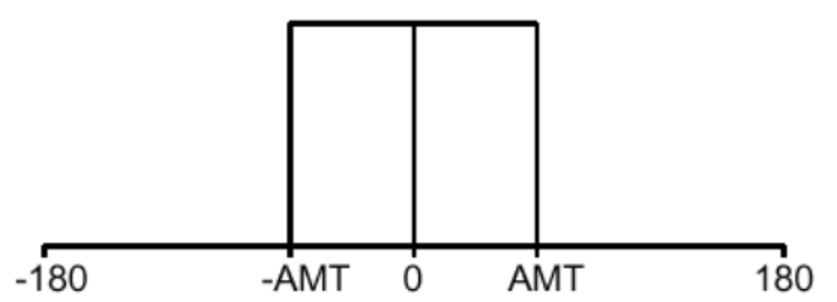
\includegraphics[scale=0.4]{Figures/UniformTADistribution.pdf}
    \subcaption{Uniform distribution} \label{sfig:Uniform}
  \end{minipage}
  \begin{minipage}[b]{0.48\textwidth}
    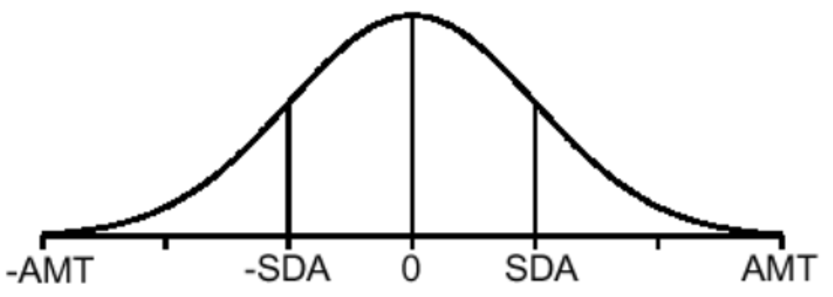
\includegraphics[scale=0.4]{Figures/NormalTADistribution.pdf}
    \subcaption{Normal distribution} \label{sfig:Normal}
  \end{minipage}
  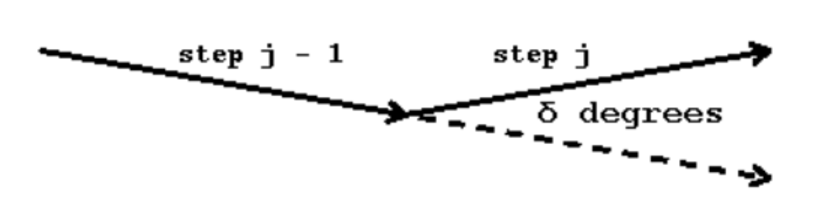
\includegraphics[scale=0.5]{Figures/TurningAngle.pdf}
  \subcaption{Example path} \label{sfig:TurningAngle}
  \end{center}
  \caption{Turning Angle for \ref{sfig:Uniform} uniform distribution,
  \ref{sfig:Normal} normal distribution, and \ref{sfig:TurningAngle} depiction
  of what a path may look like.}\label{fig:TurningAngle}
\end{figure}
{\bf Erich-Maybe in this figure we should just use the uniform distribution?}


Alternatively, if the pollinator is already at a plant, the pollinator picks a
random direction uniformly and takes a step with length $r+1$ distributed
uniformly.  This will ensure that the pollinator will not immediately return to
the same plant on the next step.

\subsection{Pollination}

When a pollinator is on a plant, it collects pollen, distributes pollen, and
consumes food. Each plant has a particular number of flowers, $\phi$, from which
a pollinator may obtain pollen. When a pollinator visits a plant it picks up
pollen from one or more flowers. The number of flowers from which a pollinator
can obtain pollen is determined by the total number of flowers on a plant, the
fraction of flowers in bloom at any one time ($a$), the number of times ($j$)
the plant has previously been visited by a pollinator, and the maximum fraction
of flowers available for pollination ($\eta$). The formula for the number of
total flowers available for visitation during a $k^{th}$ visit to the $j^{th}$
plant ($f_{j,k}$) is given by

\begin{equation}\label{flowers}
f_{j,k} = \phi \cdot a \cdot \eta^k.
\end{equation}

The amount of food eaten and the amount of pollen collected is proportional to
the number of visited flowers. Pollinators collect and eat pollen from each
flower they visit.  The amount of pollen collected and the amount of food eaten
is proportional to the equation \eqref{flowers}. Let $f^{\left(i\right)}_{j,k}$
be the number of flowers visited by the $i^{th}$ pollinator during the $k^{th}$
visit to the $j^{th}$ plant, then the amount of pollen consumed by the $i^{th}$
pollinator after $m$ plant visits is given by 
\begin{equation}
  c^{\left(i\right)}_m = \sum_{j=0}^{m} \beta f^{\left(i\right)}_{j,k},
  \label{limit} 
\end{equation} 
where $\beta$ is the proportionality constant for
the amount of pollen collected at a plant.  Each pollinator has a maximum amount
of food they will ingest, $c_{max}$, where if they eat that much food they will
stop searching. 

The fraction, $\alpha$, of all flowers are pollinated, and the associated
probability that a flower is pollinated, $\rho$, are related by the equation,
\begin{equation} \label{Prob}
  \alpha = \rho \cdot \hat{f}_k.
\end{equation}
Using equation \eqref{limit} and \eqref{Prob} we can determine the probability
that a flower is pollinated, $\rho$, by the formula
\begin{equation*}
  \rho = \frac{\alpha}{\phi} \cdot \frac{1 - \eta}{a \cdot \eta}.
\end{equation*}
To determine where the pollen originated when a flower is pollinated, we
consider each flower previously visited but exclude those flowers from the same
plant as the flower being pollinated.    Self-pollination, is not considered,
since the likelihood of self-pollination is low due to mechanisms that impedes
self-pollination. Each other flower considered has an equal likelihood of
pollinating the current flower, and a flower is chosen at random.

\subsection{Time and Stopping Criteria}

The speed a pollinator travels ($v$) is constant, as well as the time spent on a
plant ($t_{plant}$).  The travel time for a pollinator is then given by the
formula
\[
  t^{\left(i\right)} = \frac{s^{\left(i\right)}}{v} + T^{\left(i\right)} \cdot t_{plant},
\]
where $T^{\left(i\right)}$ is the number of plants visited by the $i^{th}$
pollinator. If we let the maximum allowable travel time be $t_{max}$, then once
$t^{\left(i\right)} \geq t_{max}$ or $c^{\left(i\right)}_m \geq c_{max}$ the
pollinator is removed from the simulation. $t_{max}$ is based on the optimal
searching time during the day.  When the pollinator leaves the simulation, it is
terminated.

\subsection{Model Statistics}

To best explore the inherent differences between biotic and abiotic pollination
this study focuses on the effects of the strength of the correlated random walk
as well as the effects of plant density.

\begin{table}[h]
  \centering
\setlength{\extrarowheight}{15pt}
\begin{tabular}{|l|l|}
  \hline
  % after \\: \hline or \cline{col1-col2} \cline{col3-col4} ...
  Measure & Equation \\ \hline   \hline
  Average Path Distance & $\bar{s} = \dfrac{1}{b} \nsum\limits_{i=1}^b\,
    \nsum\limits_{j=1}^n s^{\left(i\right)}_j$ \\ \hline
  \multirow{2}{*}{\parbox{0.2\textwidth}{Average Maximum \\ Distance}} &
    $\bar{M} = \dfrac{1}{b} \nnsum_{i=1}^b \max\limits_j
        \sqrt{\left(x^{\left(i\right)}_{1,0} - x^{\left(i\right)}_{1,j}\right)^2
          + \left(x^{\left(i\right)}_{2,0} - x^{\left(i\right)}_{2,j}\right)^2}$
    \\ & \\ \hline
  \multirow{2}{*}{\parbox{0.2\textwidth}{Average Pollination \\ Distance}} &
    $\bar{p} = \dfrac{1}{n} \nnsum_{i=1}^{n}
        \left(\frac{1}{\tau^{\left(i\right)}} \nsum_{j=1}^{\tau^{\left(i\right)}}
            \sqrt{\left(x^{\left(i\right)}_1 - x^{\left(j\right)}_1\right)^2
            + \left(x^{\left(i\right)}_2 - x^{\left(j\right)}_2\right)^2}
        \right)$ \\ & \\ \hline
  \multirow{2}{*}{\parbox{0.2\textwidth}{Average Maximum \\
      Pollination Distance}} &
    $\bar{P} = \dfrac{1}{n} \nnsum_{i=1}^{n} \max\limits_j
      \sqrt{\left(x^{\left(i\right)}_1 - x^{\left(j\right)}_1\right)^2
        + \left(x^{\left(i\right)}_2 - x^{\left(j\right)}_2\right)^2}$ \\ & \\ \hline
  \multirow{2}{*}{\parbox{0.2\textwidth}{Average Weighted \\ Diversity of
      Father}} &
    $E = \dfrac{1}{n} \nnsum_{i=1}^n
      \dfrac{1}{\frac{1}{\left(\tau^{\left(i\right)}\right)^2}
      \sum_{j=1}^{\Delta\tau^{\left(i\right)}} F^2_{j,i}}$ \\ & \\ \hline
\end{tabular}
\caption{Equations}
\label{tab:eqn}
\end{table}

We calculate \emph{Average Path Distance} and \emph{Average Maximum Distance},
which are based upon the pollinators' movement and gives a sense how this
movement differs with changes in density and the maximum turning angle.  We also
calculate \emph{Average Pollination Distance}, \emph{Average Maximum Pollination
Distance}, and \emph{Average Weighted Diversity of Fathers}, which are based on
the pollination events occurring in the model.  These give a more direct results
in how gene flow is affected in the model.  The calculations of these statistics
are given in the \autoref{tab:eqn}.

In these equations it is assumed that $b$ is the number of pollinators, $n$ is
the total number of plants, $(x_{1,0}^{(i)},x_{2,0}^{(i)})$ is the starting
location of the $i^{th}$ pollinator, $(x_{1,j}^{(i)},x_{2,j}^{(i)})$ is the
location of the $i^{th}$ pollinator after $j$ steps, $\tau^{(i)}$ is the total
number of seeds for the $i^{th}$ plant, $\Delta\tau^{(i)}$ is the number of
different fathers contributing pollen to the $i^{th}$ plant, and $F_{j,i}$ is
the number of times the $j^{th}$ father contributed pollen to the $i^{th}$
plant.

\section{Results}
  The following results are based on simulations of the model with parameter
values given in \autoref{tab:parameter}.  The grid size was 101 patches by 101
patches.

\begin{table}
  \begin{tabular}{|l|l|l|l|}
    \hline
    % after \\: \hline or \cline{col1-col2} \cline{col3-col4} ...
    Parameter Description & Symbol & Value &  \\ \hline  \label{parameter}
    Total number of pollinators & b & 1,000 & fixed  \\ \hline
    Maximum time & $t_{\text{max}}$ & 1,200 seconds & fixed \\ \hline
    Fraction of blooms at one time & a & 0.2 & fixed \\ \hline
    Maximum fraction of available flowers & $\eta$ & 0.75 & fixed \\ \hline
    Search radius & r & 1.0 & fixed \\ \hline
    Number of flowers per plant & $\phi$ & 100 & fixed \\ \hline
    Probability of pollination   & $\rho$ & 0.4286 & calculated \\ \hline
    Number of plants & n & 1000 & fixed \\ \hline
    Time spent at each plant & $t_{\text{plant}}$ & 100 seconds & fixed \\ \hline
  \end{tabular}
  \caption{Parameter Values}
  \label{tab:parameter}
\end{table}

The standard error was calculated by dividing the sample standard deviation by
the square root of the total number of samples.   The standard errors were all
less than 1\% on average, so will not be shown due to the small size.

Determining the distance pollinators travel during a foraging trip is important
factor for their survivability.  In order for an animal to survive it must find
enough food while foraging, without losing too much energy.  In this study the
density of plants is varied, which can directly affect the amount of foraging
the pollinators will be able to achieve in a set amount of time.  The higher the
density the greater the potential for the animal to forage.  The maximum angle
is also varied-- the relationship of this angle with respect to foraging is a
more complicated one.  In terms of foraging, a very small maximum turning angle
may not result in successful foraging due to the paths being too linear.  On the
other hand, a maximum turning angle which is too large can result in search
patterns which repetitively cover the same area over and over again.

\begin{figure}
  \begin{center}
  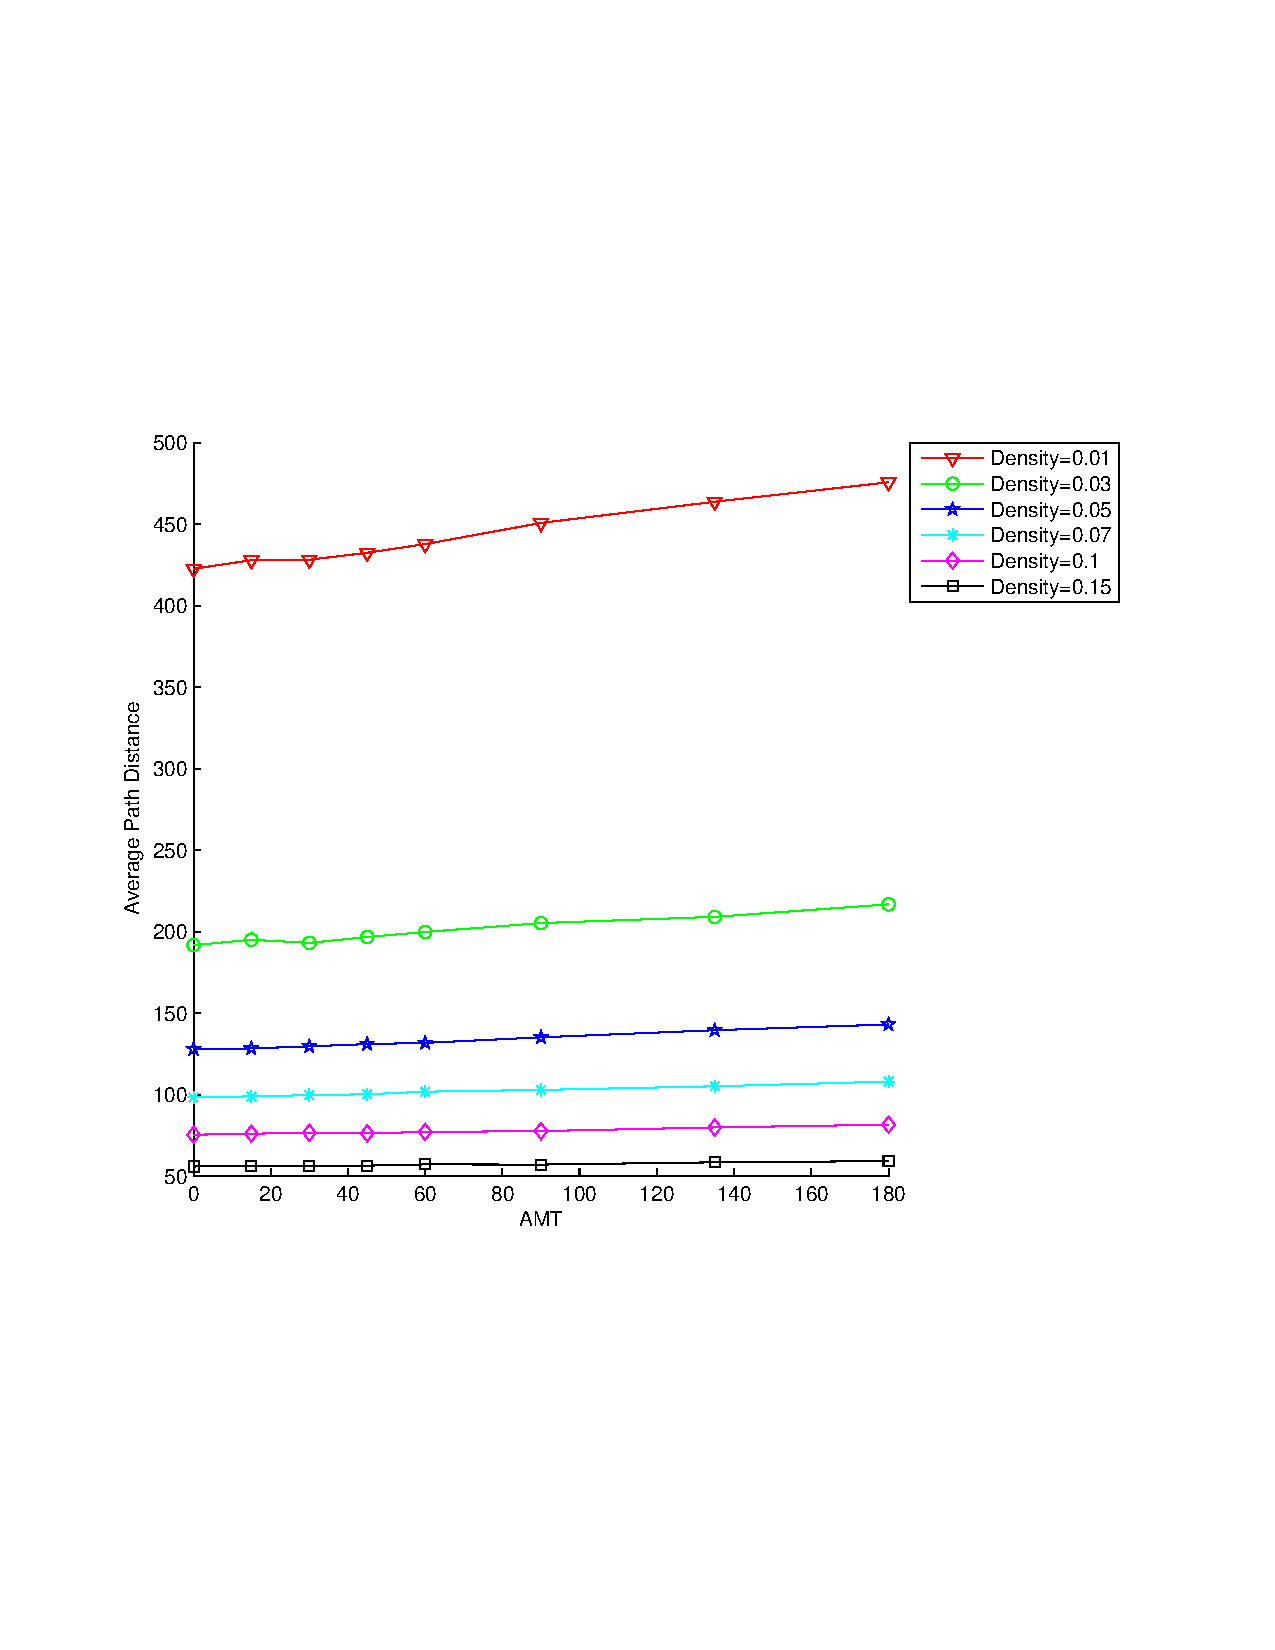
\includegraphics[scale=0.5]{PathVsAMT.pdf}
  \end{center}
  \caption{\small Average Path Distance vs. Turning Angle for Various Plant Densities}
  \label{fig:AvgPathN}
\end{figure}

In \autoref{fig:AvgPathN} the average distance traveled for each animal
decreases with increasing density due to higher foraging success.  In this
situation the pollinators will spend more time on plants, since they can find plants
more readily.  The maximum turning angle does not appear to have a large effect
on the distance.  There is a modest effect of maximum turning angle on low plant
density, where the larger the angle increases the average distance due to less
success of foraging.

The average maximum distance traveled by pollinators, see \autoref{AvgMaxDBees}, is
affected by both the turning angle and plant density. As with the average path
distance, the maximum distance decreases with higher density which decreases the
overall travel time for the pollinators.  Though in this case due to the movement
patterns the angle has a large effect on maximum distance especially at lower
densities.  As the maximum angle decreases the pollinators are more likely to travel
directly away from their starting points increasing the maximum distance
traveled.

\begin{figure}
  \begin{center}
  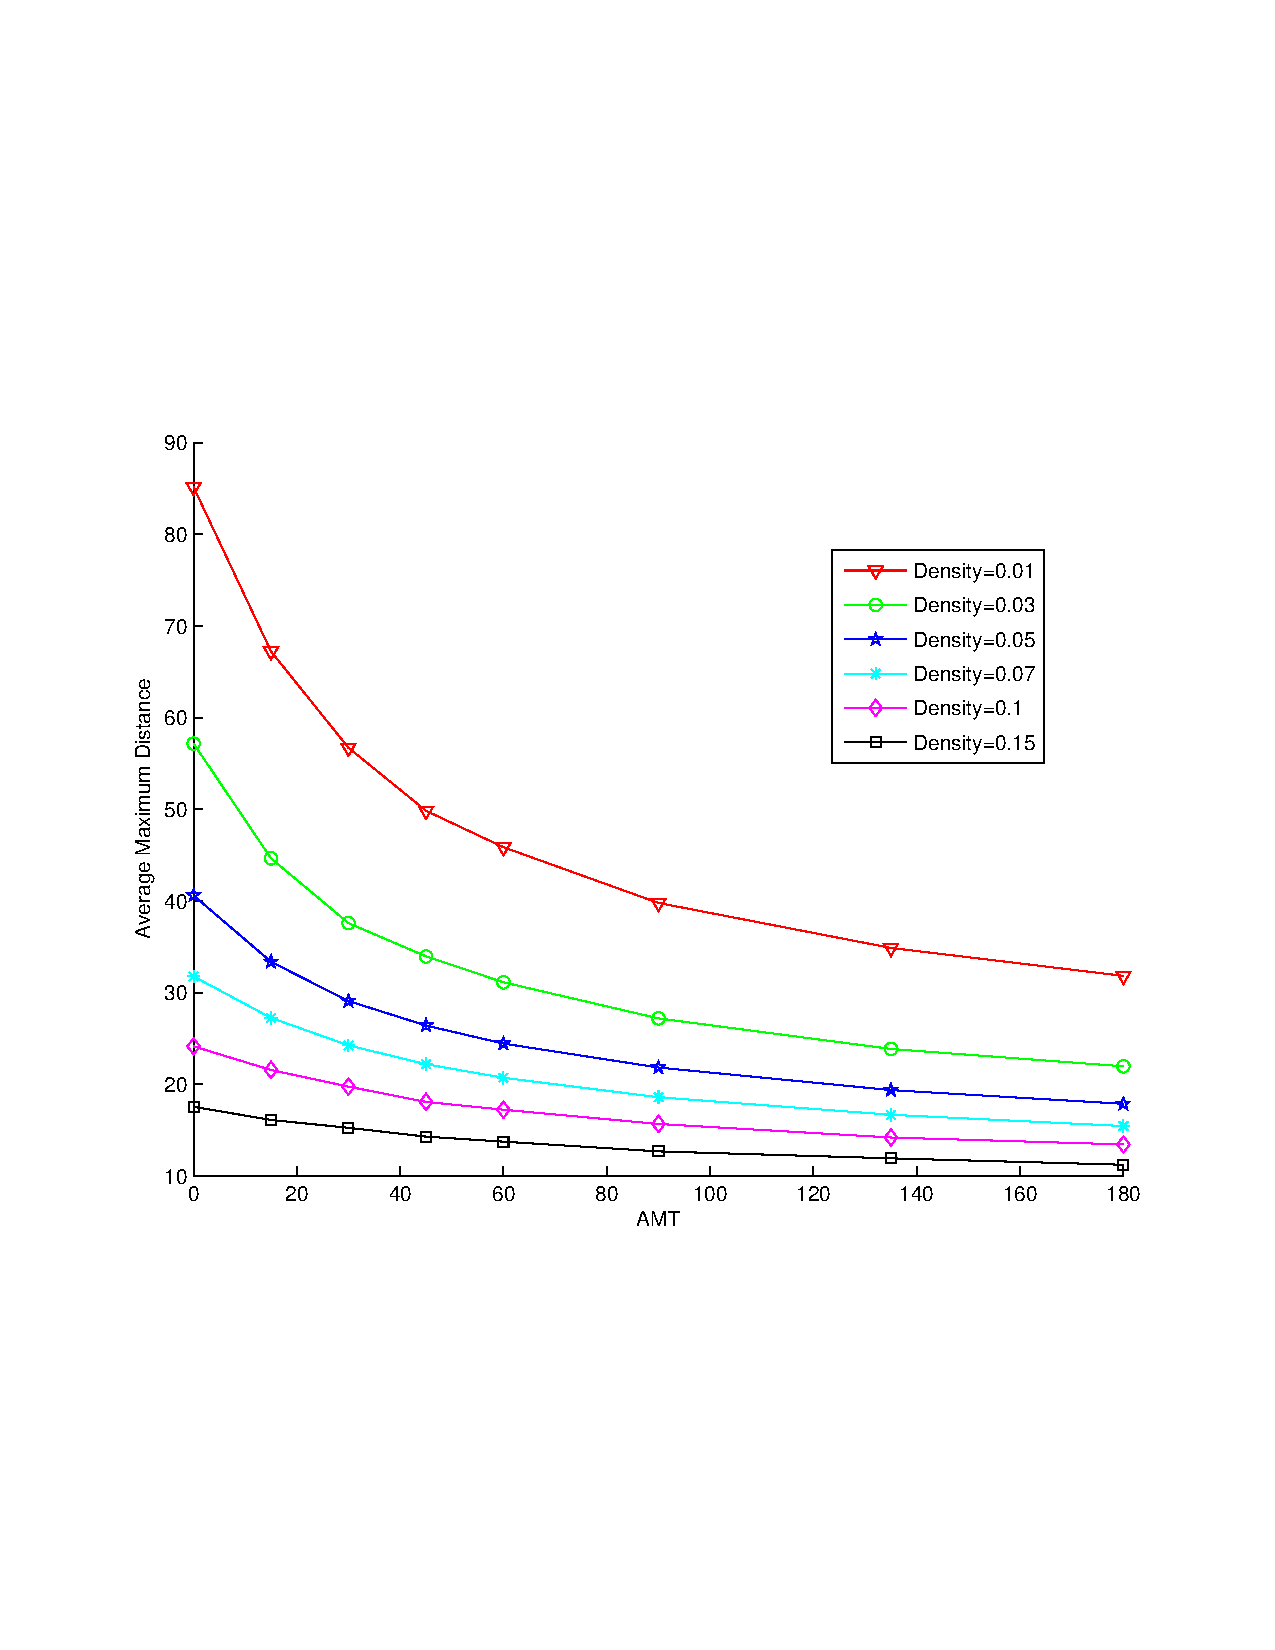
\includegraphics[scale=0.5]{MaxDVsAMT.pdf}
  \end{center}
  \caption{\small Average Maximum Distance vs. Turning Angle for Various Plant Densities}
  \label{AvgMaxDBees}
\end{figure}

For a plant density of 0.01 and AMT = $0^\circ$ the average maximum distance is
quadruple of the average maximum distance for a plant density of 0.01 and AMT =
$180^\circ$. For a higher plant density of 0.15 the average maximum distance is
50\% larger. Thus, a purely random diffusion process results in shorter average
maximum distances as compared to smaller turning angles, and as was seen with
the average pollination distance the effect of turning angle is more pronounced
for smaller plant densities. Again, this is expected since for higher plant
densities the animal direction is reset more often and therefore the animal path
becomes more and more like a purely random walk.

\begin{figure}
  \begin{center}
  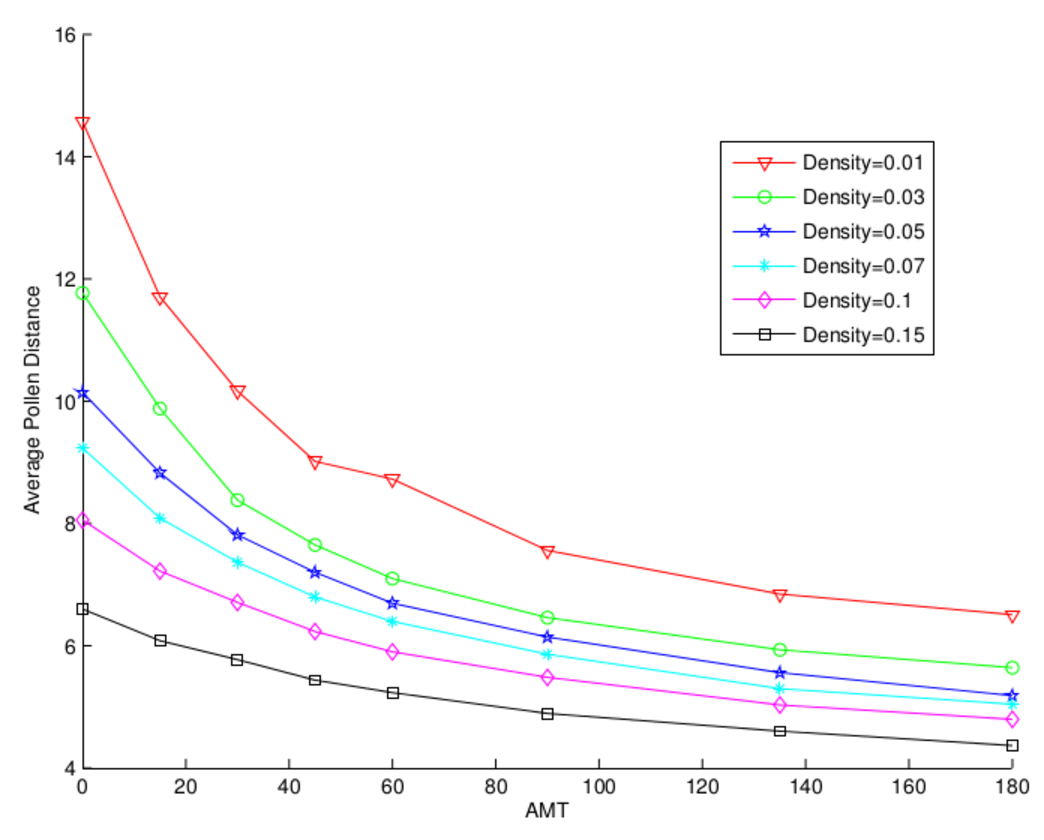
\includegraphics[scale=0.5]{PollenDVsAMT.pdf}
  \end{center}
  \caption{\small Average Pollination Distance vs. Turning Angle for Various Plant Densities}
  \label{AvgDist}
\end{figure}

The average pollination distance, see \autoref{AvgDist}, decreases with
increasing density due to the greater likelihood of pollinating nearby trees.
As with the average maximum distance, as the maximum angle decreases the animal
is likely to travel farther from its initial position which allows for longer
pollination distances.

For a plant density of 0.01 and AMT = $0^\circ$ the average maximum pollination
distance is approximately triple of that for the same plant density and AMT =
$0^\circ$. Additionally, for plant density of 0.15 and AMT = $0^\circ$ the
average pollination distance is approximately double of the average pollination
distance for the same density and AMT = $180^\circ$. Clearly, the average
pollination distance for wind dispersal is less than that of an average
pollination distance for an animal that follows a straighter path for any of the
simulated plant densities.

\begin{figure}
  \begin{center}
  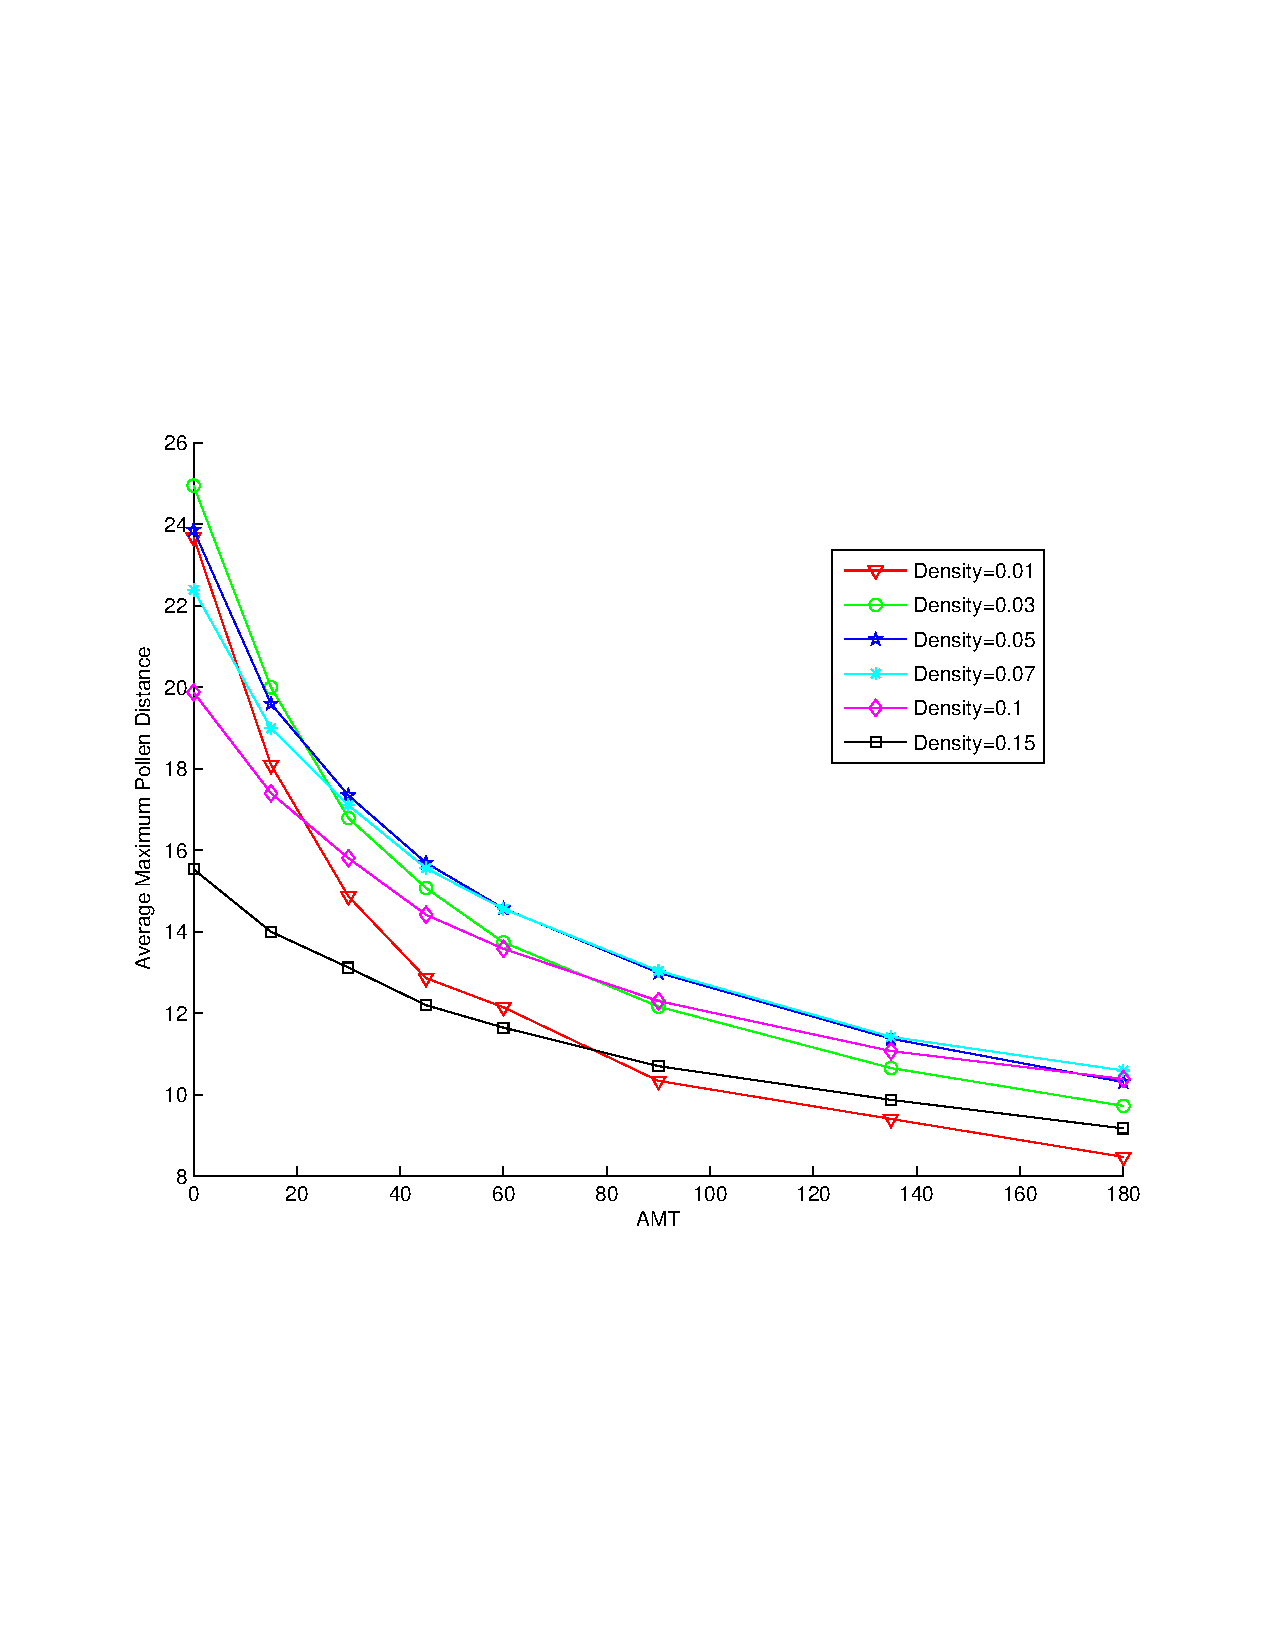
\includegraphics[scale=0.5]{MaxPollenVsAMT.pdf}
  \end{center}
  \caption{\small Average Maximum Pollination Distance vs. Turning Angle for Various Plant Densities}
  \label{AvgMaxDTreesN}
\end{figure}

The average maximum pollination distance has a much more complicated
relationship with density and maximum turning angle, see
\autoref{AvgMaxDTreesN}.  The average maximum pollination distance decreases as
maximum turning angle increases from $0^{\circ}$ to $180^{\circ}$ across all
densities.  This is due to pollinators covering a shorter distance for higher
turning angles, and therefore the plants that are visited will be closer
together on average. 

Additionally, we see that the resultant average maximum pollination distance for
a purely random diffusion process is marketably lower than those for correlated
random walks resulting in straighter animal paths. Thus, wind dispersal will
result in an average maximum pollination distance that is less than the average
maximum pollination distance for a correlated random walk. Thus, one might
expect that wind dispersal of pollen results in a smaller areal extent of gene
flow as compared to animal mediated gene flow.

The density affects the maximum pollination distance in a more complex fashion.
The higher the density the more gradual the decrease is in the maximum
pollination distance as the maximum turning angle increases.  Whereas for lower
densities this decrease is much larger.  This is likely due to the fact that at
lower densities pollination occurs less frequently with a larger variability of
maximum pollination distances.

\begin{figure}
  \begin{center}
  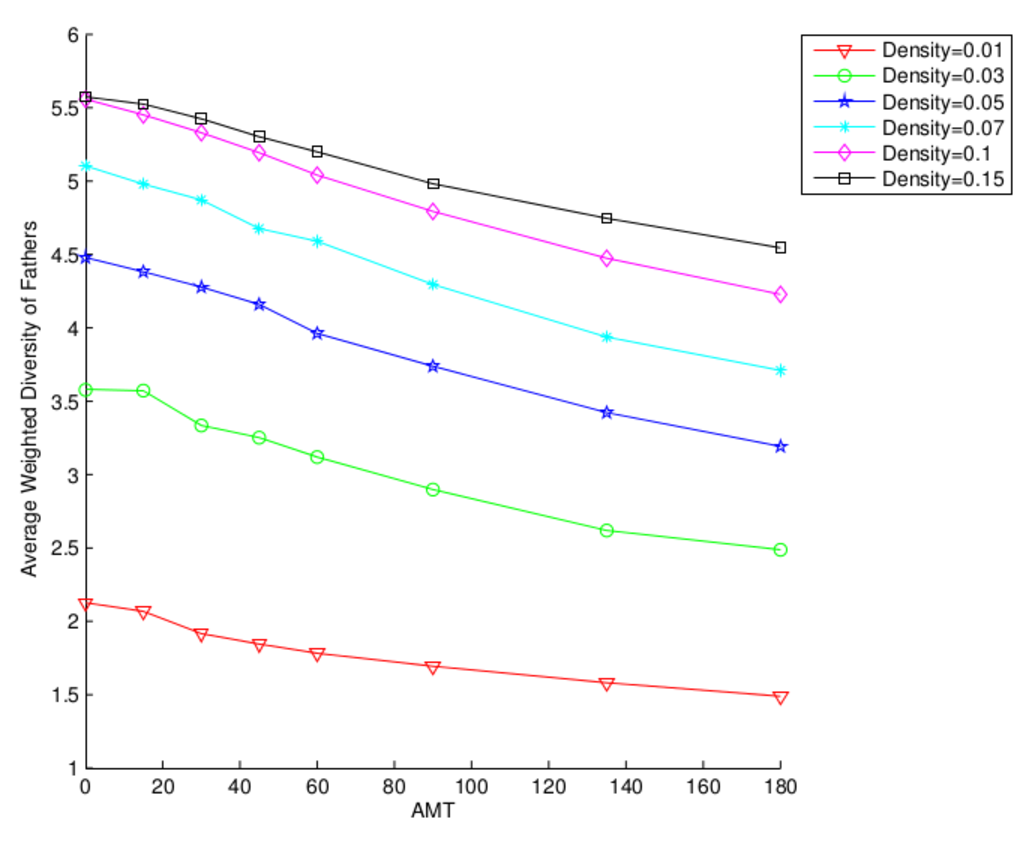
\includegraphics[scale=0.5]{WDFvsAMT.pdf}
  \end{center}
  \caption{\small Average Weighted Diversity of Fathers vs. Turning Angle for Various Plant Densities}
  \label{fig:EFathers}
\end{figure}

In general there is a small decrease in the average weighted diversity of
fathers as the maximum turning angle increases, see \autoref{fig:EFathers}. With
higher maximum turning angles the search patterns tend to be more circular,
lowering the overall diversity that a plant will see.  On the other hand, by
increasing the density, plants will see an increase in diversity due to the
larger amount of plants near by.  This effect is lessened at higher densities
due to the limited foraging time of the pollinators.

\section{Discussion}
  Pollination is a critical process to all life and is a very difficult one to
study for a variety of reasons: pollen size, pollinator diversity, plant
diversity, etc.  In this study we have used a single agent-based model with
correlated random walk to simulate both abiotic and biotic pollination.  This
simulation approach provides a powerful method for studying pollination given
the logistical difficulties associated with direct field monitoring.

A striking result is increases in pollination distances, average and maximum,
that occur with the biotic model versus the abiotic model.  In particular at
both low and high densities we observe at least 29\% and as high as 96\%
increases in the average distance pollen travels in moderately or highly
correlated random walks over the purely random walks.  For the average maximum
pollination distance the increases range from 44\% to 148\%.  This can lead to
unexpected consequences especially if say an animal pollinated, genetically
modified crop is placed a particular distance from an non-genetically modified
crop based on a purely random diffusion model.  In this situation there could be
unintended cross contamination.


The majority of models studying pollination have assumed a purely random
diffusion process. There is clear evidence that there are differences in
statistics seen between plants pollinated through wind dispersal from those
pollinated through animal dispersal \cite{LevinKerster}.  We demonstrate here
how large these differences can be.
%{\bf Add some important biology language on the consequences of these observations.}

It is clear from the results that density plays a large role in the overall gene
flow for a species.  However in most of the statistics we calculated how animals
move is also very important.  Generally the statistics are affected by movement
more at low densities and less so at high densities.
%As can be seen in the results section the magnitude of turning angle had varying degrees of effects
%over different plant densities and therefore pollination patterns predicted by a model assuming a
%purely random walk could be vastly different from a model assuming a correlated random walk.
%For
%high plant densities, the effects of correlated random walk was less pronounced than that of low
%plant densities, except for the \emph{average weighted diversity of fathers}. In the case of
%\emph{average weighted diversity of fathers} the affect of turning angle magnitudes were more
%pronounced for high densities. Therefore, although diffusion models for densely populated plant
%species may not vary greatly from models that assume a correlated random walk for \emph{average
%pollination distance} or \emph{average maximum pollination distance} they will vary significantly
%for \emph{average weighted diversity of fathers}. This has the affect of under estimating the
%diversity of pollination for high plant densities and animal dispersal as compared to similar plant
%densities and wind dispersal.

%The variation between correlated random walk and that of a purely random walk is significant at low
%plant densities for the statistics such as \emph{average maximum distance}, \emph{average
%pollination distance}, and \emph{average maximum pollination distance} and so for the case of low
%plant densities the assumption of a purely random walk may lend to bias in the analysis of
%pollination. Most studies to date have been conducted on small herbaceous plant species whose
%densities tend to be high. Even though most of the animals statistics presented were not greatly
%influenced by turning angle for high plant densities the average weighted diversity of fathers had was
%still greatly affected by the turning angle at these densities, and therefore an assumption of a
%purely random walk would be an inappropriate assumption and at any of the densities examined in this
%study. Therefore a correlated random walk may be a better approximation to animal movement.




\subsection*{Acknowledgments}
This work was performed as a component of the Masters degree for ELF.  Portions of this research were supported by a National Science Foundation grant (DEB-0640803) to RJD and DMC.  The authors would like to thank \emph{who helped out here?  Anyone of consequence?}

\bibliographystyle{amsplain}
\bibliography{PollenPaper}%xbib}
\end{document}
